
\documentclass[11pt]{article}
\usepackage[letterpaper, margin=1in]{geometry} 
\usepackage{hyperref}
\usepackage[leftcaption]{sidecap}
\sidecaptionvpos{figure}{c} %position side caption
\usepackage{lineno}
\usepackage{lipsum}
\usepackage{indentfirst}
\usepackage{pdflscape}
\usepackage{color}
\usepackage{multirow}
\usepackage[utf8]{inputenc}
\usepackage{array}
	\newcounter{rowno}
	\setcounter{rowno}{0}
\usepackage{booktabs}
\usepackage[pdftex]{graphicx}  
\usepackage{caption}
\usepackage{natbib}
\usepackage{authblk}
\usepackage[table]{xcolor} %for table line color alteration
\usepackage{subscript}
\usepackage{longtable}
\usepackage{fancyhdr}
	\renewcommand{\headrulewidth}{0pt}
	\rfoot{\thepage}
\fancyhf{}
\renewcommand{\headrulewidth}{0pt}

\pagestyle{fancy}

\begin{document}

\centering{Table S1: Accessions of \emph{Zea mays} ssp. \emph{mexicana} (RIMME) and \emph{Zea mays} ssp. \emph{parviglumis} (RIMPA) sampled. RIHY is a \emph{Z. mays} ssp. \emph{parviglumis} and \emph{Zea mays} ssp. \emph{mays} hybrid.}

% Appendix S1. Parv and mex samples 
\begin{scriptsize}  % Switch from 12pt to 11pt; otherwise, table won't fit
\rowcolors{1}{gray!25}{white}
\begin{longtable}{>{\stepcounter{rowno}}cccccc}
\hiderowcolors
\hline
\multicolumn{1}{c}{\textbf{Accession}} & \multicolumn{1}{c}{\textbf{USDA ID}} & \multicolumn{1}{c}{\textbf{Population}} & \multicolumn{1}{c}{\textbf{Alleles Sampled}} & \multicolumn{1}{c}{\textbf{\emph{Hopscotch} Freq.}} & \multicolumn{1}{c}{\textbf{No \emph{Hopscotch} Freq.}} \\
\hline
\endhead
\showrowcolors
    RIHY0009 & N/A   & N/A   & 2     & 0.5   & 0.5 \\
    RIMME0006 & 566673 & Durango & 2	& 0 & 1 \\
    RIMME0007 & 566680 & Guanajuato & 2 & 0 & 1 \\
    RIMME0008 & 566681 & Michoacan & 2 & 0 & 1 \\
    RIMME0009 & 566682 & Distrito Federal & 2 & 0 & 1 \\
    RIMME0011 & 566685 & Mexico & 2     & 0     & 1 \\
    RIMME0014 & 714151 & Breeders line & 6     & 0     & 1 \\
    RIMME0017 & 699874 & Ayotlan & 8     & 0     & 1 \\
    RIMME0021 & N/A   & El Porvenir & 69    & 0.17 & 0.83 \\
    RIMME0026 & N/A   & Opopeo & 42    & 0.07 & 0.93 \\
    RIMME0028 & N/A   & Puruandiro & 28    & 0.04 & 0.96 \\
    RIMME0029 & N/A   & Ixtlan & 35    & 0     & 1 \\
    RIMME0030 & N/A   & San Pedro & 27    & 0     & 1 \\
    RIMME0031 & N/A   & Tenango del Aire & 25    & 0.08  & 0.92 \\
    RIMME0032 & N/A   & Nabogame & 24    & 0     & 1 \\
    RIMME0033 & N/A   & Puerta Encantada & 25    & 0     & 1 \\
    RIMME0034 & N/A   & Santa Clara & 23    & 0     & 1 \\
    RIMME0035 & N/A   & Xochimilco & 25    & 0     & 1 \\
    RIMPA0001 & 87168 & El Salado & 4     & 0     & 1 \\
    RIMPA0003 & 87171 & Mazatlan & 8 & 0.13 & 0.87 \\
    RIMPA0017 & 87200 & N/A   & 4     & 0     & 1 \\
    RIMPA0019 & 87213 & El Salado & 2     & 0.50   & 0.50 \\
    RIMPA0029 & 87244 & N/A   & 2     & 0.50   & 0.50 \\
    RIMPA0031 & 87249 & N/A   & 2     & 0.5   & 0.5 \\
    RIMPA0035 & 87288 & Jalisco & 4     & 0     & 1 \\
    RIMPA0040 & 288185 & Mexico & 4     & 0     & 1 \\
    RIMPA0042 & 288187 & Guerrero & 4     & 0.25  & 0.75 \\
    RIMPA0043 & 288188 & Guerrero & 4     & 0     & 1 \\
    RIMPA0045 & 288193 & Guerrero & 4     & 0     & 1 \\
    RIMPA0055 & 714152 & Breeders line & 2     & 0     & 1 \\
    RIMPA0056 & 714153 & Breeders line & 2     & 0.50   & 0.50 \\
    RIMPA0057 & 714154 & Breeders line & 2     & 0.50   & 0.50 \\
    RIMPA0058 & N/A   & N/A   & 4     & 0.50   & 0.50 \\
    RIMPA0059 & N/A   & N/A   & 4     & 1     & 0 \\
    RIMPA0060 & 714157 & Breeders line & 2     & 0     & 1 \\
    RIMPA0061 & 714158 & Breeders line & 4     & 0.5   & 0.5 \\
    RIMPA0062 & 714159 & Breeders line & 4     & 0.5   & 0.5 \\
    RIMPA0063 & 714160 & Breeders line & 4     & 0     & 1 \\
    RIMPA0064 & 714161 & Breeders line & 3     & 0     & 1 \\
    RIMPA0065 & 714162 & Breeders line & 4     & 0.25  & 0.75 \\
    RIMPA0068 & 699861 & Jalisco, Mexico & 16    & 0     & 1 \\
    RIMPA0069 & 699862 & Ixtlan & 14    & 0.14 & 0.86 \\
    RIMPA0070 & 699863 & Benito Jaurez & 16    & 0     & 1 \\
    RIMPA0071 & 699864 & Tuzantla & 28    & 0     & 1 \\
    RIMPA0072 & 699865 & Tiquicheo & 16    & 0     & 1 \\
    RIMPA0073 & 699866 & Tiquicheo & 16    & 0.12 & 0.88 \\
    RIMPA0074 & 699867 & Huetamo & 12    & 0     & 1 \\
    RIMPA0075 & 699868 & Huetamo & 2     & 0     & 1 \\
    RIMPA0076 & 699869 & Huetamo & 4     & 0     & 1 \\
    RIMPA0077 & 699870 & Caracuaro & 2     & 0     & 1 \\
    RIMPA0078 & 699871 & Caracuaro & 2     & 0.5   & 0.5 \\
    RIMPA0079 & 699872 & Villa Madero & 14    & 0     & 1 \\
    RIMPA0080 & 699873 & Guachinango & 12    & 0     & 1 \\
    RIMPA0081 & 699875 & Ameca & 16    & 0     & 1 \\
    RIMPA0083 & 699877 & Tepoztlan & 14    & 0     & 1 \\
    RIMPA0084 & 699878 & Tepoztlan & 16    & 0     & 1 \\
    RIMPA0085 & 699879 & Miahuatlan & 16    & 0     & 1 \\
    RIMPA0086 & 699880 & Miahuatlan & 16    & 0.06 & 0.94 \\
    RIMPA0087 & 699881 & Tecoanapa & 24    & 0     & 1 \\
    RIMPA0089 & 699883 & Guerrero & 12    & 0     & 1 \\
    RIMPA0090 & 699884 & Guerrero & 10    & 0     & 1 \\
    RIMPA0091 & 699885 & Guerrero & 16    & 0     & 1 \\
    RIMPA0092 & 699886 & Guerrero & 10    & 0     & 1 \\
    RIMPA0093 & 699887 & Guerrero & 26    & 0.08 & 0.92 \\
    RIMPA0094 & 699888 & Guerrero & 2     & 0     & 1 \\
    RIMPA0095 & 699889 & Guerrero & 4     & 0     & 1 \\
    RIMPA0096 & 699890 & Guerrero & 26    & 0.04 & 0.96 \\
    RIMPA0097 & 699891 & Guerrero & 6     & 0     & 1 \\
    RIMPA0098 & 699892 & Guerrero & 4     & 0     & 1 \\
    RIMPA0099 & 699893 & Guerrero & 4     & 0     & 1 \\
    RIMPA0100 & 699894 & Guerrero & 6     & 0     & 1 \\
    RIMPA0101 & 699895 & Guerrero & 2     & 0     & 1 \\
    RIMPA0103 & 699897 & Guerrero & 2     & 0     & 1 \\
    RIMPA0104 & 699898 & Guerrero & 22    & 0.09 & 0.91 \\
    RIMPA0105 & 699899 & Guerrero & 6     & 0     & 1 \\
    RIMPA0106 & 699900 & Guerrero & 6     & 0.33 & 0.67 \\
    RIMPA0107 & 699901 & Guerrero & 4     & 0     & 1 \\
    RIMPA0108 & 699902 & Guerrero & 6     & 0     & 1 \\
    RIMPA0109 & 699903 & Michoacan & 4     & 0.25  & 0.75 \\
    RIMPA0110 & 699904 & Michoacan & 2     & 0     & 1 \\
    RIMPA0111 & 699905 & Michoacan & 4     & 0     & 1 \\
    RIMPA0112 & 699906 & Michoacan & 4     & 0.25  & 0.75 \\
    RIMPA0114 & 699908 & Michoacan & 6     & 0.17 & 0.83 \\
    RIMPA0116 & 699910 & Mexico & 2     & 0     & 1 \\
    RIMPA0117 & 699911 & Mexico & 4     & 0     & 1 \\
    RIMPA0118 & 699912 & Mexico & 6     & 0.17 & 0.83 \\
    RIMPA0119 & 699913 & Mexico & 2     & 0     & 1 \\
    RIMPA0120 & 699914 & Mexico & 1     & 1     & 0 \\
    RIMPA0121 & 699915 & Mexico & 2     & 0     & 1 \\
    RIMPA0128 & 699922 & Mexico & 2     & 0.5   & 0.5 \\
    RIMPA0129 & 699923 & Michoacan & 2     & 0.5   & 0.5 \\
    RIMPA0135 & 699929 & Nayarit & 24    & 0     & 1 \\
    RIMPA0138 & 699932 & Jalisco & 2     & 0.5   & 0.5 \\
    RIMPA0139 & 699933 & Jalisco & 1     & 1     & 0 \\
    RIMPA0142 & 699936 & Colima & 18    & 0.44 & 0.56 \\
    RIMPA0144 & 699938 & Jalisco & 2     & 1     & 0 \\
    RIMPA0145 & 699939 & Michoacan & 1     & 1     & 0 \\
    RIMPA0147 & 699941 & Jalisco & 1     & 1     & 0 \\
    RIMPA0155 & N/A   & Jalisco & 73    & 0.01 & 0.99 \\
    RIMPA0156 & N/A   & Jalisco & 20    & 0     & 1 \\
    RIMPA0157 & N/A   & Jalisco & 58    & 0.34 & 0.66 \\
    RIMPA0158 & N/A   & Jalisco & 64    & 0.53 & 0.47 \\
    RIMPA0159 & N/A   & Jalisco & 26    & 0     & 1 \\
    RIMPA0162 & 21785 & N/A   & 4     & 0     & 1 \\
    \hline
\end{longtable}
\end{scriptsize}
\clearpage


% Appendix S2. Mays sampling

\centering{Table S2: \emph{Hopscotch} frequency in sampled \emph{Zea mays} ssp. \emph{mays} (RIMMA).}

\begin{scriptsize}  % Switch from 12pt to 11pt; otherwise, table won't fit
\rowcolors{1}{gray!25}{white}
\begin{longtable}{>{\stepcounter{rowno}}cccc}
\hiderowcolors
\hline
\multicolumn{1}{c}{\textbf{Accession}} & \multicolumn{1}{c}{\textbf{USDA ID}} & \multicolumn{1}{c}{\textbf{Alleles Sampled}} & \multicolumn{1}{c}{\textbf{\emph{Hopscotch} Freq.}} \\
\hline
\endhead
\showrowcolors
    RIMMA0066 & 27096 & 2     & 1 \\
    RIMMA0075 & 19309 & 2     & 1 \\
    RIMMA0077 & 19313 & 2     & 1 \\
    RIMMA0079 & 19321 & 2     & 1 \\
    RIMMA0081 & 20190 & 2     & 1 \\
    RIMMA0084 & 22439 & 2     & 1 \\
    RIMMA0086 & 22748 & 2     & 1 \\
    RIMMA0088 & 22756 & 2     & 1 \\
    RIMMA0089 & 23392 & 2     & 1 \\
    RIMMA0090 & 23423 & 2     & 1 \\
    RIMMA0092 & 23427 & 4     & 1 \\
    RIMMA0094 & 23447 & 4     & 1 \\
    RIMMA0097 & 23488 & 2     & 1 \\
    RIMMA0099 & 23509 & 2     & 1 \\
    RIMMA0100 & 23518 & 2     & 1 \\
    RIMMA0101 & 23519 & 2     & 1 \\
    RIMMA0104 & 24590 & 2     & 1 \\
    RIMMA0108 & 26022 & 2     & 1 \\
    RIMMA0111 & 26770 & 6     & 1 \\
    RIMMA0115 & 26798 & 2     & 1 \\
    RIMMA0117 & 27045 & 2     & 1 \\
    RIMMA0130 & 28336 & 2     & 1 \\
    RIMMA0133 & 8581 & 2     & 1 \\
    RIMMA0134 & 22632 & 2     & 1 \\
    RIMMA0135 & 22634 & 2     & 1 \\
    RIMMA0142 & 30060 & 2     & 0.5 \\
    RIMMA0143 & 30065 & 4     & 1 \\
    RIMMA0146 & 30863 & 4     & 1 \\
    RIMMA0149 & 30869 & 2     & 1 \\
    RIMMA0152 & 32722 & 2     & 1 \\
    RIMMA0153 & 32728 & 2     & 1 \\
    RIMMA0154 & 32732 & 2     & 1 \\
    RIMMA0155 & 42809 & 2     & 1 \\
    RIMMA0156 & 42872 & 2     & 1 \\
    RIMMA0157 & 42874 & 2     & 1 \\
    RIMMA0158 & 42875 & 2     & 1 \\
    RIMMA0159 & 42878 & 2     & 1 \\
    RIMMA0160 & 65864 & 2     & 1 \\
    RIMMA0162 & 65866 & 2     & 1 \\
    RIMMA0166 & 213696 & 2     & 1 \\
    RIMMA0167 & 213697 & 2     & 1 \\
    RIMMA0168 & 213698 & 2     & 1 \\
    RIMMA0169 & 213699 & 2     & 1 \\
    RIMMA0172 & 213705 & 2     & 1 \\
    RIMMA0174 & 213708 & 4     & 1 \\
    RIMMA0177 & 213715 & 2     & 1 \\
    RIMMA0178 & 213716 & 2     & 1 \\
    RIMMA0179 & 213717 & 2     & 1 \\
    RIMMA0181 & 213719 & 2     & 1 \\
    RIMMA0183 & 213721 & 2     & 1 \\
    RIMMA0184 & 213722 & 2     & 1 \\
    RIMMA0186 & 213724 & 2     & 1 \\
    RIMMA0187 & 213725 & 1     & 1 \\
    RIMMA0188 & 213727 & 2     & 1 \\
    RIMMA0195 & 213781 & 2     & 1 \\
    RIMMA0196 & 213793 & 2     & 1 \\
    RIMMA0197 & 214197 & 2     & 1 \\
    RIMMA0198 & 214293 & 2     & 1 \\
    RIMMA0199 & 214294 & 2     & 1 \\
    RIMMA0200 & 214295 & 2     & 1 \\
    RIMMA0202 & 217407 & 2     & 1 \\
    RIMMA0203 & 217408 & 2     & 1 \\
    RIMMA0206 & 217473 & 2     & 1 \\
    RIMMA0208 & 218005 & 2     & 1 \\
    RIMMA0209 & 218195 & 2     & 1 \\
    RIMMA0210 & 219871 & 2     & 1 \\
    RIMMA0212 & 219882 & 2     & 1 \\
    RIMMA0213 & 219883 & 2     & 1 \\
    RIMMA0214 & 219884 & 2     & 1 \\
    RIMMA0217 & 221872 & 2     & 1 \\
    RIMMA0218 & 221873 & 2     & 1 \\
    RIMMA0220 & 221876 & 2     & 1 \\
    RIMMA0221 & 221877 & 2     & 1 \\
    RIMMA0222 & 221878 & 2     & 1 \\
    RIMMA0223 & 221880 & 2     & 1 \\
    RIMMA0226 & 221889 & 2     & 1 \\
    RIMMA0227 & 222314 & 2     & 1 \\
    RIMMA0228 & 222315 & 2     & 1 \\
    RIMMA0229 & 222316 & 2     & 1 \\
    RIMMA0230 & 222317 & 2     & 1 \\
    RIMMA0232 & 222469 &  2     & 1 \\
    RIMMA0233 & 222470 & 2     & 1 \\
    RIMMA0235 & 222474 & 2     & 0.5 \\
    RIMMA0242 & 222614 & 2     & 1 \\
    RIMMA0243 & 222615 & 2     & 1 \\
    RIMMA0247 & 222639 & 4     & 1 \\
    RIMMA0248 & 222640 & 2     & 1 \\
    RIMMA0249 & 222641 & 2     & 1 \\
    RIMMA0252 & 233002 & 2     & 1 \\
    RIMMA0253 & 233006 & 2     & 1 \\
    RIMMA0254 & 233008 & 2     & 1 \\
    RIMMA0256 & 237000 & 2     & 1 \\
    RIMMA0257 & 257506 & 2     & 1 \\
    RIMMA0258 & 267179 & 2     & 1 \\
    RIMMA0259 & 269743 & 2     & 1 \\
    RIMMA0260 & 269744 & 2     & 1 \\
    RIMMA0262 & 270297 & 2     & 1 \\
    RIMMA0263 & 278713 & 2     & 1 \\
    RIMMA0264 & 278716 & 2     & 1 \\
    RIMMA0265 & 278717 & 2     & 1 \\
    RIMMA0268 & 278721 & 2     & 1 \\
    RIMMA0269 & 278724 & 2     & 1 \\
    RIMMA0270 & 280061 & 2     & 1 \\
    RIMMA0272 & 280853 & 2     & 1 \\
    RIMMA0275 & 311232 & 2     & 1 \\
    RIMMA0276 & 311235 & 2     & 1 \\
    RIMMA0277 & 311236 & 2     & 1 \\
    RIMMA0279 & 311241 & 2     & 1 \\
    RIMMA0280 & 311243 & 2     & 1 \\
    RIMMA0283 & 401757 & 2     & 1 \\
    RIMMA0285 & 414176 & 2     & 1 \\
    RIMMA0288 & 452032 & 2     & 1 \\
    RIMMA0290 & 452045 & 2     & 1 \\
    RIMMA0291 & 452046 & 2     & 1 \\
    RIMMA0292 & 452047 & 2     & 1 \\
    RIMMA0293 & 452048 & 2     & 1 \\
    RIMMA0298 & 483273 & 2     & 1 \\
    RIMMA0302 & 540784 & 2     & 1 \\
    RIMMA0305 & 548792 & 2     & 1 \\
    RIMMA0310 & 550462 & 2     & 1 \\
    RIMMA0312 & 550466 & 2     & 1 \\
    RIMMA0320 & 583896 & 2     & 1 \\
    RIMMA0322 & 583898 & 2     & 1 \\
    RIMMA0324 & 587125 & 2     & 1 \\
    RIMMA0334 & 587153 & 2     & 1 \\
    RIMMA0336 & 607519 & 2     & 1 \\
    RIMMA0337 & 607522 & 2     & 1 \\
    RIMMA0338 & 607593 & 2     & 1 \\
    RIMMA0339 & 607599 & 2     & 1 \\
    RIMMA0340 & 607602 & 2     & 1 \\
    RIMMA0341 & 608465 & 2     & 1 \\
    RIMMA0342 & 608502 & 2     & 1 \\
    RIMMA0344 & 608539 & 2     & 1 \\
    RIMMA0346 & 608618 & 2     & 1 \\
    RIMMA0347 & 608619 & 2     & 1 \\
    RIMMA0350 & 608646 & 2     & 1 \\
    RIMMA0351 & 608652 & 2     & 1 \\
    RIMMA0352 & 608764 & 2     & 1 \\
    RIMMA0357 & 608777 & 2     & 1 \\
    RIMMA0360 & N/A & 18    & 1 \\
    RIMMA0362 & N/A & 8     & 1 \\
    RIMMA0363 & N/A & 16    & 1 \\
    RIMMA0370 & N/A & 17    & 1 \\
    RIMMA0372 & N/A & 24    & 1 \\
    RIMMA0373 & N/A & 22    & 1 \\
    RIMMA0408 & 478967 & 2     & 1 \\
    RIMMA0411 & 479044 & 1     & 1 \\
    RIMMA0413 & 484413 & 1     & 1 \\
    RIMMA0414 & 484421 & 1     & 1 \\
    RIMMA0424 & 485120 & 8     & 0.9 \\
    RIMMA0432 & 489126 & 1     & 1 \\
    RIMMA0434 & 490921 & 2     & 0.5 \\
    RIMMA0435 & 490973 & 1     & 1 \\
    RIMMA0442 & 537097 & 2     & 1 \\
    RIMMA0443 & 537099 & 2     & 1 \\
    RIMMA0444 & 538009 & 2     & 1 \\
    RIMMA0445 & 538011 & 2     & 1 \\
    RIMMA0446 & 539920 & 2     & 1 \\
    RIMMA0447 & 539921 & 2     & 1 \\
    RIMMA0448 & 539922 & 2     & 1 \\
    RIMMA0449 & 539923 & 2     & 1 \\
    RIMMA0450 & 539924 & 2     & 1 \\
    RIMMA0451 & 539926 & 2     & 1 \\
    RIMMA0452 & 539927 & 2     & 1 \\
    RIMMA0453 & 543843 & 2     & 1 \\
    RIMMA0454 & 543846 & 2     & 1 \\
    RIMMA0455 & 543847 & 2     & 1 \\
    RIMMA0456 & 543849 & 2     & 1 \\
    RIMMA0457 & 543850 & 2     & 1 \\
    RIMMA0458 & 547086 & 2     & 1 \\
    RIMMA0459 & 547088 & 2     & 1 \\
    RIMMA0483 & 600954 & 2     & 1 \\
    RIMMA0490 & 601003 & 2     & 1 \\
    RIMMA0515 & 601270 & 2     & 1 \\
    RIMMA0537 & 601416 & 2     & 1 \\
    RIMMA0550 & 601468 & 2     & 1 \\
    RIMMA0553 & 601489 & 2     & 1 \\
    RIMMA0559 & 601495 & 2     & 1 \\
    RIMMA0561 & 601497 & 2     & 1 \\
    RIMMA0562 & 601498 & 2     & 1 \\
    RIMMA0571 & 601562 & 2     & 1 \\
    RIMMA0572 & 601563 & 2     & 1 \\
    RIMMA0577 & 601568 & 2     & 1 \\
    RIMMA0579 & 601570 & 2     & 1 \\
    RIMMA0590 & 601724 & 2     & 1 \\
    RIMMA0591 & 601725 & 2     & 1 \\
    RIMMA0592 & 601729 & 2     & 1 \\
    RIMMA0593 & 601773 & 2     & 1 \\
    RIMMA0594 & 601774 & 2     & 1 \\
    RIMMA0595 & 601775 & 2     & 1 \\
    RIMMA0596 & 601776 & 2     & 1 \\
    RIMMA0597 & 601777 & 2     & 1 \\
    RIMMA0598 & 601778 & 2     & 1 \\
    RIMMA0599 & 601779 & 2     & 1 \\
    RIMMA0600 & 601780 & 2     & 1 \\
    RIMMA0601 & 601781 & 2     & 1 \\
    RIMMA0602 & 601782 & 2     & 1 \\
    RIMMA0603 & 601783 & 2     & 1 \\
    RIMMA0604 & 601784 & 2     & 1 \\
    RIMMA0605 & 601785 & 2     & 1 \\
    RIMMA0606 & 601786 & 2     & 1 \\
    RIMMA0607 & 601787 & 2     & 1 \\
    RIMMA0608 & 601788 & 2     & 1 \\
    RIMMA0609 & 601789 & 2     & 1 \\
    RIMMA0610 & 601790 & 2     & 1 \\
    RIMMA0611 & 601791 & 2     & 1 \\
    RIMMA0612 & 601792 & 2     & 1 \\
    RIMMA0613 & 601808 & 2     & 1 \\
    RIMMA0622 & 645837 & 2     & 0.5 \\
    RIMMA0624 & 645930 & 1     & 1 \\
    RIMMA0629 & 646057 & 2     & 0.5 \\
    RIMMA0631 & 646072 & 2     & 0.5 \\
    RIMMA0659 & 286729 & 2     & 1 \\
    RIMMA0660 & 485451 & 2     & 1 \\
    RIMMA0678 & 285833 & 1     & 1 \\
    RIMMA0681 & 628446 & 2     & 1 \\
    RIMMA0683 & 483568 & 2     & 1 \\
    RIMMA0684 & 28482 & 2     & 1 \\
    RIMMA0685 & 287623 & 4     & 1 \\
    RIMMA0693 & 487959 & 2     & 1 \\
    RIMMA0694 & 28487 & 2     & 1 \\
    RIMMA0695 & 28567 & 1     & 1 \\
    RIMMA0699 & 28465 & 2     & 1 \\
    RIMMA0704 & 28623 & 2     & 1 \\
    RIMMA0706 & 28615 & 2     & 1 \\
    RIMMA0711 & 29075 & 1     & 1 \\
    RIMMA0713 & 489399 & 2     & 1 \\
    RIMMA0715 & 28454 & 2     & 1 \\
    RIMMA0717 & 483926 & 2     & 1 \\
    RIMMA0718 & 484805 & 2     & 1 \\
    RIMMA0723 & 28565 & 2     & 1 \\
    RIMMA0724 & 490826 & 2     & 1 \\
    RIMMA0725 & 490827 & 1     & 1 \\
    RIMMA0728 & 484969 & 1     & 1 \\
    RIMMA0732 & 28456 & 2     & 1 \\
    RIMMA0734 & 26028 & 2     & 1 \\
    RIMMA0738 & N/A & 2     & 1 \\
    RIMMA0739 & N/A & 2     & 1 \\
    RIMMA0744 & N/A & 2     & 1 \\
    RIMMA0747 & N/A & 1     & 1 \\
    RIMMA0748 & N/A & 2     & 1 \\
    RIMMA0749 & N/A & 2     & 1 \\
    RIMMA0750 & N/A & 2     & 0.5 \\
    RIMMA0751 & N/A & 1     & 1 \\
    RIMMA0752 & N/A & 1     & 1 \\
    RIMMA0753 & N/A & 2     & 1 \\
    RIMMA0755 & N/A & 2     & 1 \\
    \hline
\end{longtable}
\end{scriptsize}

\clearpage

% Appendix S3. Cartoon representation of tb1 locus
%-------------------------------------------------------------------
%\begin{figure*}[!t]
  %\begin{center}
   %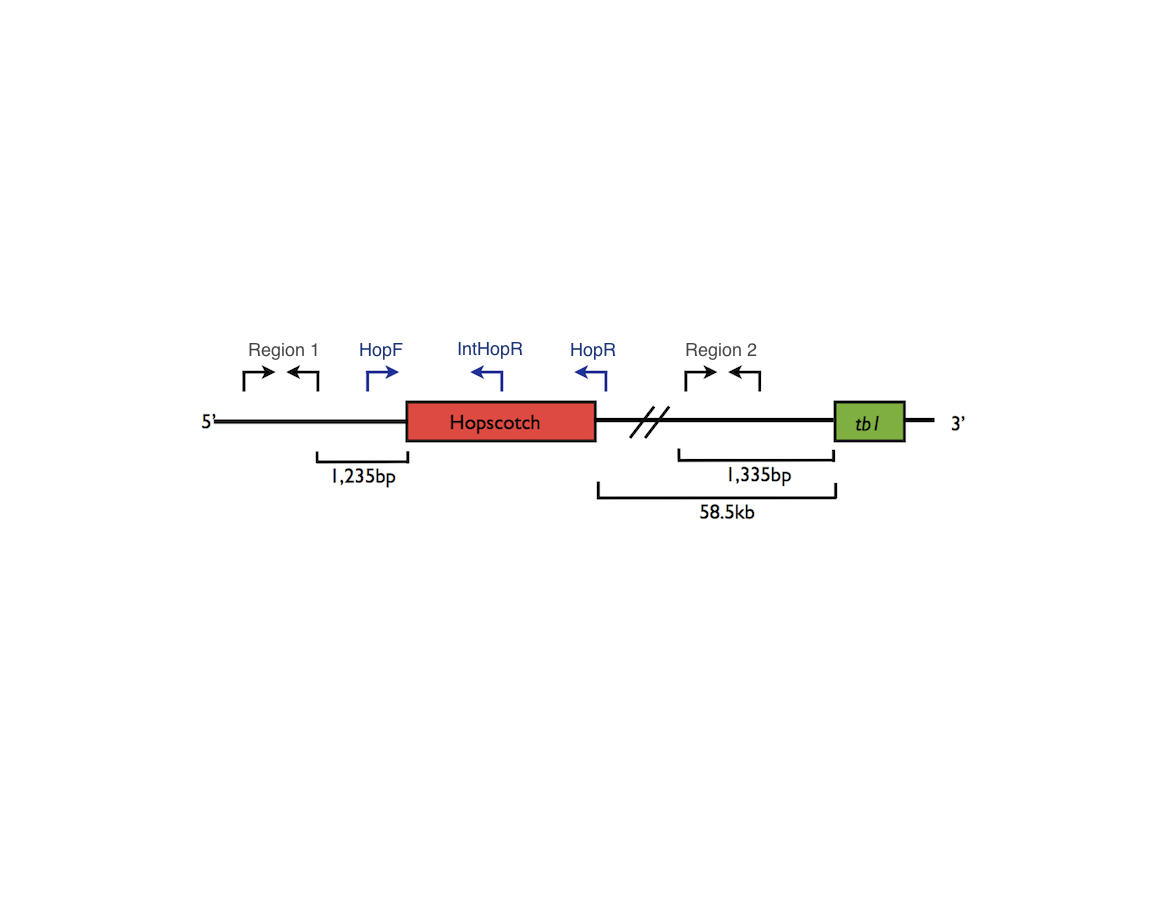
\includegraphics[width=180mm]{FigS1LocusCartoon.png}
   %\flushleft{Figure S1: Representation of the upstream regulatory region of \emph{tb1}, showing the \emph{tb1} coding region (green) and the \emph{Hopscotch} insertion (red). Arrows show the location of primer sets; in black, primers used for amplification and sequencing (Region 1; within the 5' UTR, and Region 2; 66,169 bp upstream from the tb1 ORF); in blue, primers used to genotype the \emph{Hopscotch} insertion.}
  %\end{center}
%\end{figure*}
%-------------------------------------------------------------------

\clearpage


% Appendix S4. Gel image
%-------------------------------------------------------------------
\begin{figure*}[!t]
  \begin{center}
   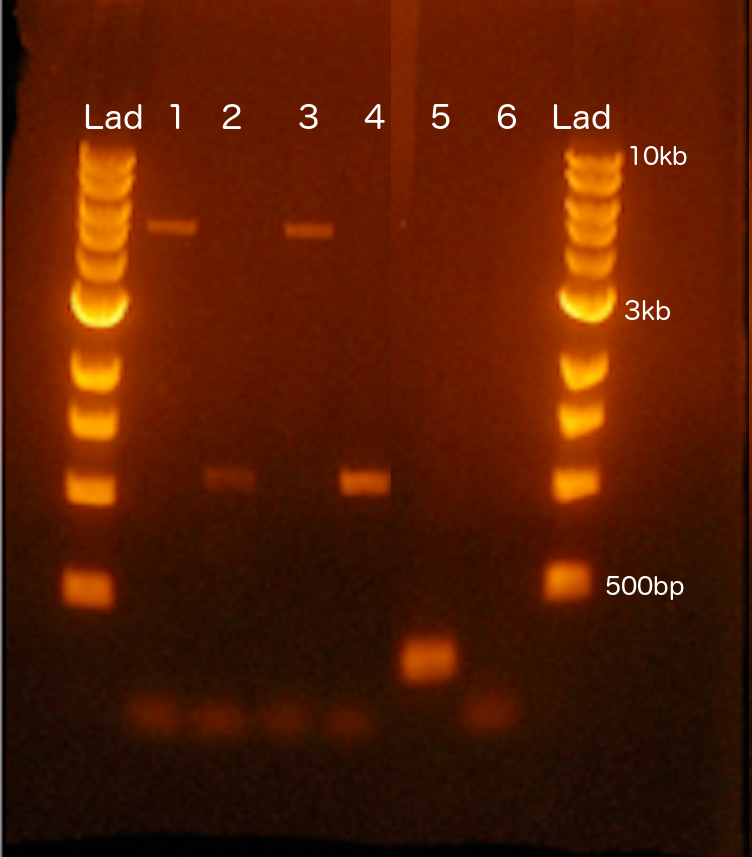
\includegraphics[width=100mm]{FigS2GelPeerJ_pretty.png}
   \flushleft{Figure S1: Agarose gel image of amplification products for genotyping of the \emph{Hopscotch} element. Lanes 1 (HopF/HopR; 5kb band) and 2 (HopF/HopIntR; 1.1kb) are the products for one individual that is homozygous for the element; Lanes 3 (HopF/HopR; 5kb band) and 4 (HopF/HopIntR; 1.1kb) are also the products of an individual that is homozygous for the element; and Lanes 5 (HopF/HopR; 300bp) and 6 (HopF/HopIntR; N/A) are the products of an individual that is homozygous for the teosinte (lacking the \emph{Hopscotch}) allele.} 
  \end{center}
\end{figure*}
%-------------------------------------------------------------------

\clearpage


% Appendix S5. NJ Trees
%-------------------------------------------------------------------
\begin{figure*}[!t]
  \begin{center}
   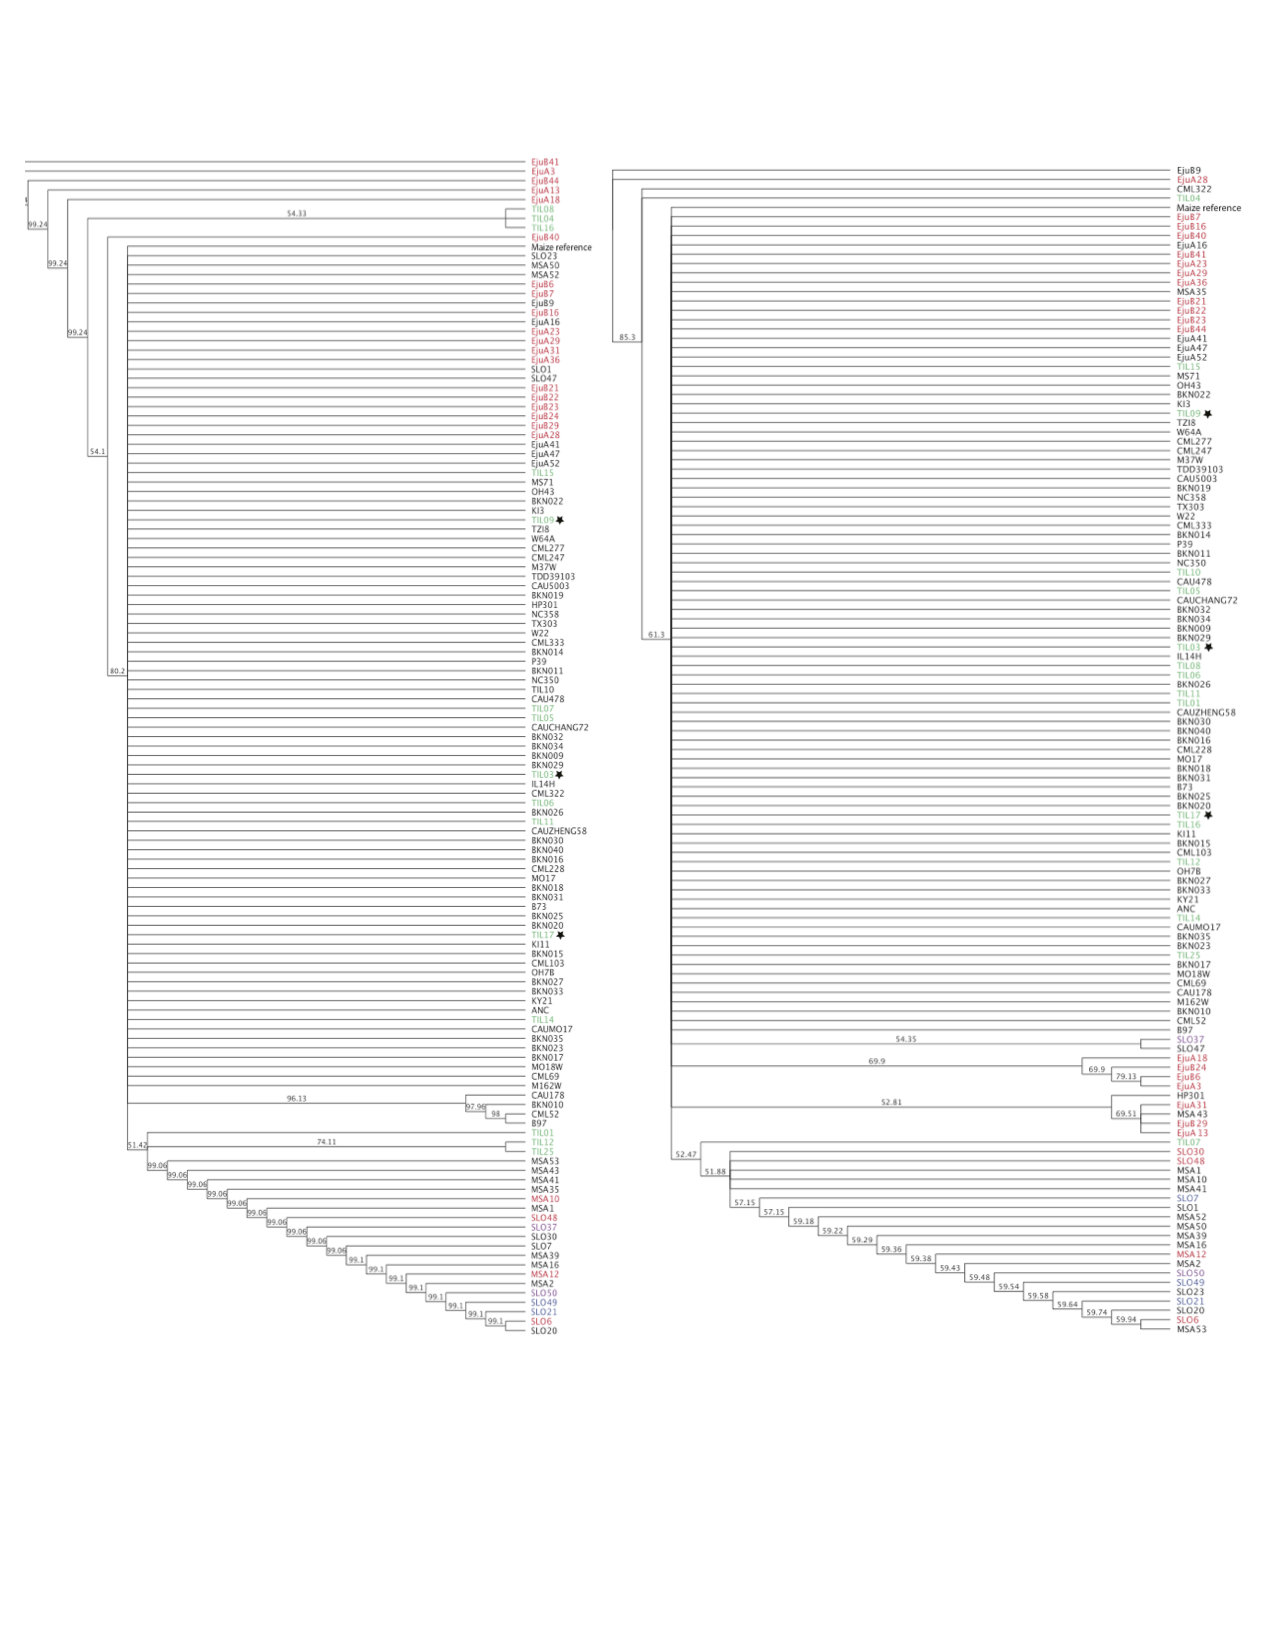
\includegraphics[width=150mm]{FigS3NJtrees.png}
    \flushleft{Figure S2: Neighbor-joining tree of the sequenced region in the 5' UTR (right; Region 1) and the 66,169 bp upstream region (left; Region 2) of \emph{tb1}. Individuals with genotype data are colored: Homozygous for the teosinte (no \emph{Hopscotch}) allele (red), homozygous for the maize (\emph{Hopscotch}) allele (blue), heterozygotes (purple). TILs (teosinte inbred lines) are colored in green, with stars indicating the 3 TILs known to have the \emph{Hopscotch} insertion. Black indicates individuals not genotyped for the \emph{Hopscotch} insertion. EjuA refers to individuals from population Ejutla A, EjuB from Ejutla B, SLO from San Lorenzo, and MSA from La Mesa. Remaining individuals are lines of maize (\emph{Zea mays} ssp. \emph{mays}).}  

\end{center}
\end{figure*}
%-------------------------------------------------------------------
\end{document}
